\subsection{Exemplars}
In this section, the current IT-systems will be described and what other systems that can be used to plan what food to eat.
Ideas from other existing systems will be found and put into the context of this projects system. \fxnote{CHS: Still don't know how to incorporate metaphors}

\subsubsection{Food Planner}
One technology that are currently being used to make a food plan is a mobile application called \textit{Food Planner}.
In this application the users can plan meals ahead of time, lookup recipes, look at what groceries that needs to be bought, list what the user have in the fridge and appends bought items to the fridge.
The following section will take a look at the application, in order to find ideas which will be good in the context of this projects system.

\begin{figure}[H]
    \centering
    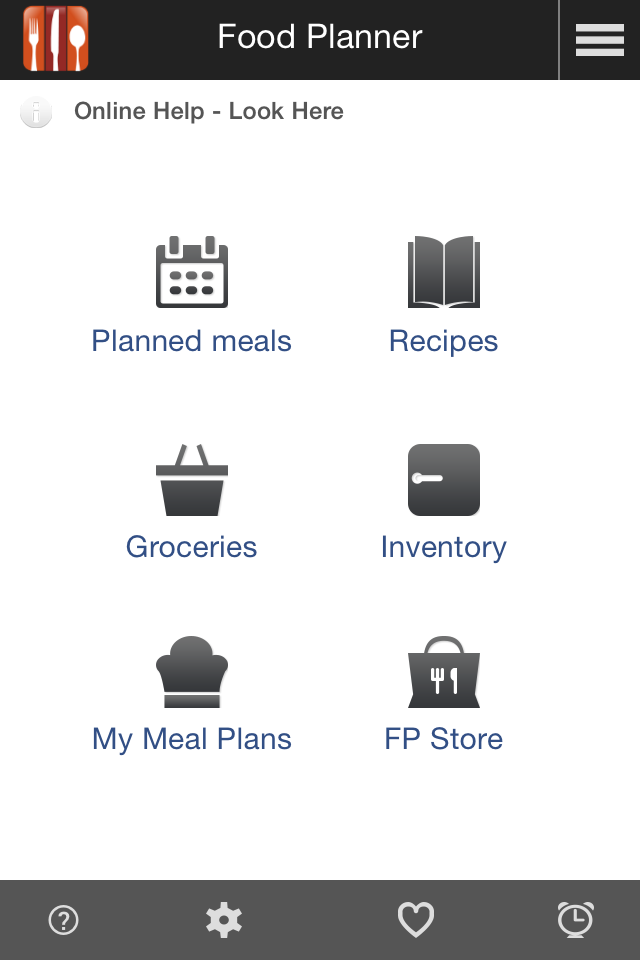
\includegraphics[width=0.5\textwidth]{Grafik/FoodPlanner/index}
    \caption{An image displaying the index of the application Food Planner}
    \label{FoodPlannerIndex}
\end{figure}

\textbf{Useful ideas:}
\begin{itemize}
  \item \textbf{Inventory:} Each product can be added separately, and the application can be used to keep track on the amount
  \item \textbf{Recipes:} Custom recipes can be created through the application, or they can be found/bought in the application store, or the internet, either by a Google search, or following a link directly to known websites, with recipes.
  \item \textbf{My meal plans:} This menu can keep track of meal plans, that has been added to the application.
  \item \textbf{Planned meals:} In this menu the upcoming days can be planed, with multiple recipes each day, either by adding them manually, or by adding a meal plan from \textit{My meal plans}. Missing groceries for a desired number of days ahead, can then automatically be added to a \textit{Grocery menu}.
  \item \textbf{Registering:} By registering with an e-mail and a password, the application allows the user to back up the information, synchronizing with other devises and sharing is also enabled.
  \item \textbf{Grocery menu:} Here, groceries that needs to be bought, can be added either automatically from \textit{My meal plan} or added manually. If an item is not known to the program, it can be added using a bar-code scanner, and naming the item manually.
\end{itemize}
\fxnote{Will add more pics of Food Planner app.}

\textbf{Ideas used in our context}
\begin{itemize}
  \item \textbf{Inventory:} To help avoiding food waste, this idea would be useful. By prioritizing the inventory, the food in the home, has a better chance of being used, before it expires.
  \item \textbf{Recipes:} Using Recipes, people can try new meals, and if the ingredients list, needed for the meal is known, the Inventory can be taken into account, or a list of needed ingredients can be added to the grocery menu.
  \item \textbf{My meal plans:} With this idea, it is easy to save different diets, and lists of favourite meals, etc.
  \item \textbf{Planned meals:} Knowing what food is planned ahead, new recipes can be added to reduce food waste and/or variate the meals.
  \item \textbf{Registering:} This idea enables the use of synchronizing, which could be useful if the program is used in a household of more than one, or if it is to be used on multiple devices.
  \item \textbf{Grocery menu:} This menu is very useful, for the use of a shopping list, where it can be tracked what has been bought and what still needs to be bought.
\end{itemize}

\subsubsection{Website\fxnote{To be rewritten, do not read yet!}}
Another alternative could be a tool found on the website madplanuge.dk\cite{madSpild_madPlanUge}. This tool is a basic food planner, where the food plan can be planned one week ahead, but the users storage is taken into consideration.

When the user enters the website the user can either choose between 20 random recipes or search for something the user would like to eat.
Then the user can choose up to 3 recipes for each of the days so the user can plan breakfast, lunch and dinner for each specific day.
After the food plan has been selected, the user can then get a shopping list of all the needed items.
If the user creates a user on the site, the user will be able to save, and favorite different recipes.
If the user finds a recipe with some ingredients who the user likes, would the user be able to get more recipes based upon those ingredients.

\begin{figure}[H]
    \centering
    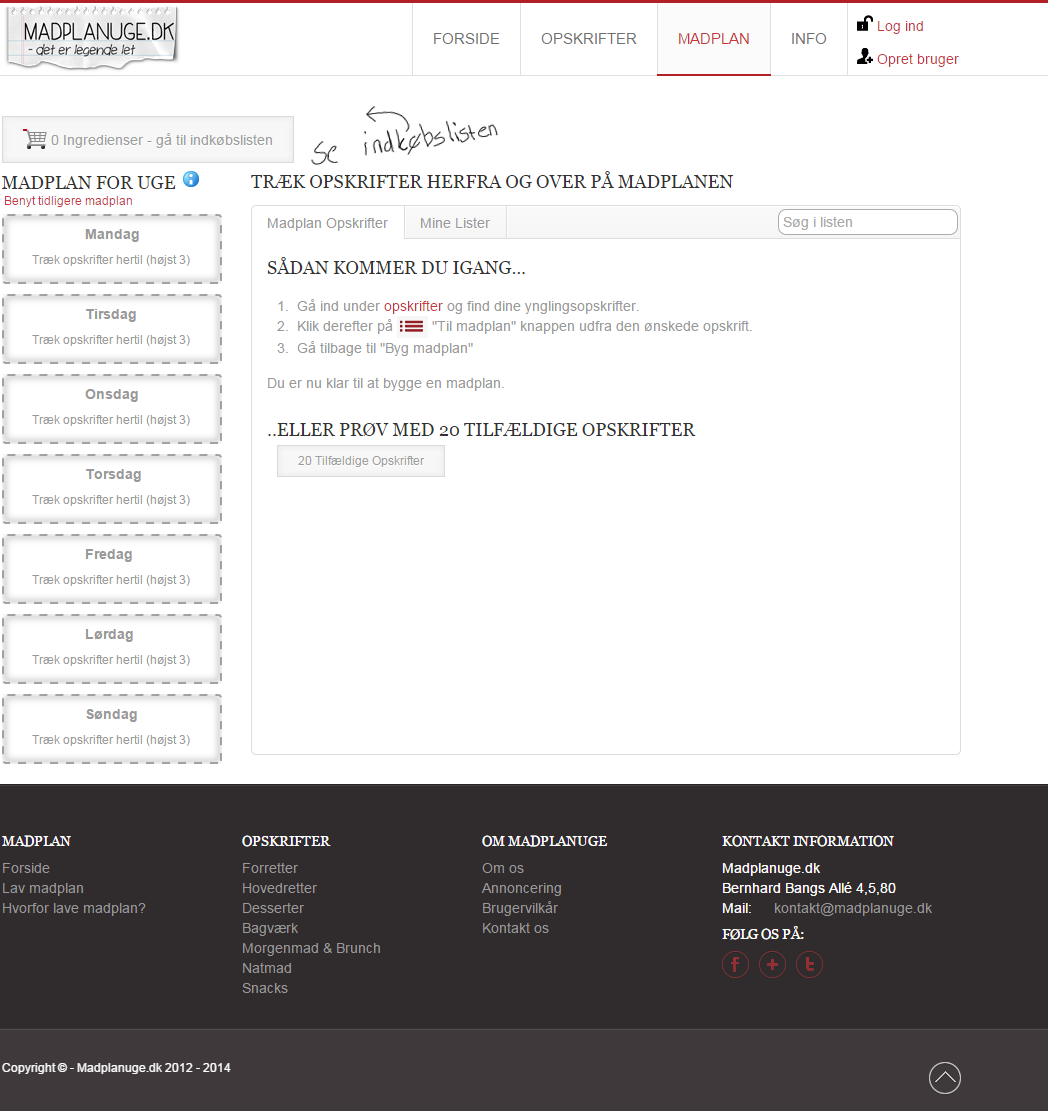
\includegraphics[width=0.5\textwidth]{Grafik/madplanuge}
    \caption{An image displaying the the website Madplan Uge}
    \label{MadPlanUge}
\end{figure}
